%%%%%%%%%%%%%%%%%%%%%%%%%%%%%%%%%%%%%%%%%%%%%%%%%%%%%%%%%%%%%%%%
\fbox{
\begin{minipage}[c]{.5\linewidth}
	\section*{Força  [N] [Kgf]}
	\large
	$\begin{array}{ l l l l l }
		\sum F_{(t)} & = & M \; a_{(t)} & = & M \; \ddot{x}_{(t)}
	\end{array}$
	\newline
	\newline
	$\begin{array}{ l l l }
		\sum F_{R} & = & \sum F_{action} \; - \; \sum F_{reaction}
	\end{array}$
	\newline
	\newline
	$\begin{array}{ l l l }
		f_{(t)} & = & -K \; x_{(t)} \\
		f_{(t)} & = & -B \; \dot{x}_{(t)}
	\end{array}$
	\newline
	\newline
	\newline
	%%%There are only forces if there is a physical object subject to them.
\end{minipage}
}
%\newline
\hspace{.1cm}
%\newline
\fbox{
\begin{minipage}[c]{.5\linewidth}
	\section*{Torque [N.m]}
	\large
	$\begin{array}{ l l l l l }
		\sum T_{(t)} & = & J \; \gamma_{(t)} & = & M \; \ddot{\theta}_{(t)}
	\end{array}$
	\newline
	\newline
	$\begin{array}{ l l l }
		\sum T_{R} & = & \sum T_{action} \; - \; \sum T_{reaction}
	\end{array}$
	\newline
	\newline
	$\begin{array}{ l l l }
		T_{(t)} & = & -K \; \theta_{(t)} \\
		T_{(t)} & = & -B \; \dot{\theta}_{(t)} \\
		T & = & F \times r
	\end{array}$
	\newline
	\newline
	%%%Never mix potatoes with bananas.
\end{minipage}
}
\newline
\vspace{.6cm}
\newline
\begin{minipage}[c]{.5\linewidth}
	\section*{Energia [Joule]}
	\vspace{.1cm}
	\Large
	$\begin{array}{ l l l }
		W & = & F \; d \\
		W & = & P \; \Delta t \\
		E & = & M \; C^{2}
	\end{array}$
\end{minipage}
\begin{minipage}[c]{.5\linewidth}
	\begin{figure}[H]
		\flushleft
		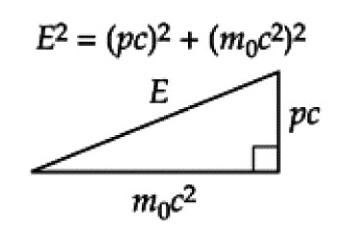
\includegraphics[scale=0.6]{./image/General/Einstein.jpg}
		\caption*{\cite{book-2}}
		\label{Einstein}
	\end{figure}
\end{minipage}
\newline
\vspace{.6cm}
\newline
\begin{minipage}[!b]{.5\linewidth}
	\section*{Energia Cinética [Joule]}
	\Large
	$\begin{array}{ l l l }
		E_{c} & = & \frac{1}{2} \; m \; v^{2}
	\end{array}$
\end{minipage}
\begin{minipage}[!b]{.5\linewidth}
	\section*{Energia Potencial [Joule]}
	\Large
	$\begin{array}{ l l l }
		E_{p} & = & \; m \; g \; h
	\end{array}$
\end{minipage}
\newline
\vspace{.6cm}
\newline
\begin{minipage}[l]{\linewidth}
	\section*{Energia Térmica}
	\Large
	$\begin{array}{ l l l l }
		Q - Heat \quad energy & & & \\
		Q_{(t)} - temperature & & & \\
		R - heat \quad resistance & & & \\
		& Q & = & \frac{Q_{1(t)} - Q_{2(t)}}{R}
	\end{array}$
\end{minipage}
%%%%%%%%%%%%%%%%%%%%%%%%%%%%%%%%%%%%%%%%%%%%%%%%%%%%%%%%%%%%%%%%
%%%%%%%%%%%%%%%%%%%%%%%%%%%%%%%%%%%%%%%%%%%%%%%%%%%%%%%%%%%%%%%%
%%%%%%%%%%%%%%%%%%%%%%%%%%%%%%%%%%%%%%%%%%%%%%%%%%%%%%%%%%%%%%%%
\begin{comment}
\newline
\vspace{1cm}
\newline
$\frac{A \times B}{C}\times D \approx E$,
\newline
\begin{minipage}{0pt}
	$$\begin{array}{l | l}
		\text{Média aritmetica dados classificados} & \text{Variância de uma amostra dados classificados} \\
		\overline{x} = \frac{1}{n}\sum_{i=1}^cx_in_i = \sum_{i=1}^cx_if_i & s^2 = \frac{1}{n-1}\sum_{i=1}^c (x_i-\bar{x})^2 n_i
	\end{array}$$
\end{minipage}
\newline
\vspace{1cm}
\newline
$IC_{1-\alpha}=\left[ A, B\right]$ ; para $1-\alpha = 0.95$, $\alpha=0.05$, $\frac{\alpha}{2}=0.025$
\newline
\vspace{1cm}
\newline
Zona critica $Z_c=Z_{1-\frac{\alpha}{2}}=\Phi^{-1}(0.975) \cong 1.96$
\newline
\vspace{1cm}
\newline
$P\left( A \leqslant \mu \leqslant B \right) = 1-\alpha$ \\
$\triangle=Z_c\times\frac{\delta}{\sqrt{n}}$ \\
$A = \bar{x}-\triangle \qquad and \qquad B = \bar{x}+\triangle$ \\
$\therefore$\\
$IC_{A_{0.95}}=\left[ \; 18.8877 \: , \: 21.1956 \; \right]$ \hspace{1cm} and \hspace{1cm} $IC_{B_{0.95}}=\left[ \; 20.4519 \: , \: 22.6314 \; \right]$
\newline
\vspace{1cm}
\newline
$\left[ \; \mu \; \right]$
\newline
\vspace{1cm}
\newline
$\bar{y}_{A_0}$ = 6,6111 \qquad $\bar{y}_{B_0}$ = 7,5111 \qquad $n=90$ \\
$\delta_A$ = 2,3112 \qquad $\delta_B$ = 2,5140
\newline
\vspace{1cm}
\newline
$P(Y_A < 6)=P(Y_A \leqslant 5)=F_{i_B}(5) \cong 0,3677 $  \quad e \quad $P(Y_B < 6)=P(Y_B \leqslant 5)=F_{i_B}(5) \cong 0,2444$ \\
\newline
\vspace{1cm}
\newline
$\hat{P_A}-\hat{P_B} \sim N \left( p_A - p_B ; \frac{p_A\:q_A}{n_A} + \frac{p_B\:q_B}{n_B}\right)$ \hspace{1cm}
$\triangle=z_{(1-\frac{\alpha}{2})} \;\sqrt{\frac{\hat{p_A} \: \hat{q_A}}{n_A}+\frac{\hat{p_B} \: \hat{q_B}}{n_B}}$ \hspace{1cm} $q=(1-p)$
\newline
\vspace{1cm}
\newline
$IC_{97\%}(\hat{P_A}-\hat{P_B})=\left[(\hat{p_A}-\hat{p_B})-\triangle \: ; \: (\hat{p_A}-\hat{p_B})+\triangle \right]$
\newline
\vspace{1cm}
\newline
$\hat{P_A}-\hat{P_B} \sim N \left( 0,1233 \; ; \; 0,02788\right)$ \hspace{1cm}
$z_{(1-\frac{\alpha}{2})}=\phi^{-1}(0,985)=2,1701$
\newline
\vspace{1cm}
\newline
Recorrendo a calculadora casio $fx-9860GII$ :
\newline
\vspace{1cm}
\newline
$\triangle= InvNorm(0.985)\sqrt{\frac{0.3677(1-0.3677)}{90}+\frac{0.2444(1-0.2444)}{90}}\: \cong \:0.3677$
\\
$\therefore$
\\
$IC_{97\%}(\hat{P_A}-\hat{P_B})=\left[ \; (\hat{p_A}-\hat{p_B}) \:-\: 0,3624 \: ; \: (\hat{p_A}-\hat{p_B}) \:+\: 0,3624 \; \right]$
\newline
\vspace{1cm}
\newline
\begin{minipage}[l]{0pt}
	$$\left\lbrace\begin{array}{l}
		H_0: \quad \mu_A-\mu_B=0 \\
		\\
		H_1: \quad \mu_A-\mu_B<0
	\end{array}\right.$$
\end{minipage}
\newline
\vspace{1cm}
\newline
\begin{minipage}[l]{0pt}
	$$\left\lbrace\begin{array}{c}
		\mu \;=\; 0 \\
		\delta \;=\; s \\
	\end{array}\right.$$
\end{minipage}
\hspace{3cm} $\Longrightarrow$ \hspace{1cm}
\begin{minipage}[l]{0pt}
	\[\bar{X}=\bar{X}_A-\bar{X}_B \quad \backsim N \left( 0\:,\: \frac{\delta_A^2}{n_A}+\frac{\delta_B^2}{n_B} \right) \quad ; \quad \frac{\delta_A^2}{n_A}+\frac{\delta_B^2}{n_B}\;\cong0.6558 \]
\end{minipage}
\newline
\vspace{1cm}
\newline
$P(\bar{X}_{H_0} \leqslant C)=0.05 \quad \implies \quad RC_X\left] -\infty \:,\: -1.332 \right] \qquad \bar{x}_A-\bar{x}_B=-1.5 \in RC_X $
\newline
\vspace{1cm}
\newline
\begin{minipage}[l]{0pt}
	\[  z_0\:=\: \frac{\bar{x}_A-\bar{x}_B}{\sqrt{\frac{\delta_A^2}{n_A}+\frac{\delta_B^2}{n_B}}}\:\cong\: -1.8523 \qquad
	RC_z \:=\: \left] -\infty \:,\: -1.6448 \right]  \qquad
	pvalue \:=\: P(Z<z_0) \:=\: 0.032 \]
\end{minipage}
\newline
\vspace{1cm}
\newline
\hspace*{5cm} \underline{Condição NEE:}\\
\begin{minipage}[l]{0pt}
	$$\left\lbrace\begin{array}{c}
		\mu \;=\; 0 \\
		\delta \;=\; s \\
	\end{array}\right.$$
\end{minipage}
\hspace{3cm} $\Longrightarrow$ \hspace{1cm}
\begin{minipage}[l]{0pt}
	\[ \bar{Y}=\bar{Y_A}-\bar{Y_B} \quad \backsim N \left( 0\:,\: \frac{\delta_A^2}{n_A}+\frac{\delta_B^2}{n_B} \right) \quad ; \quad \frac{\delta_A^2}{n_A}+\frac{\delta_B^2}{n_B} \; \cong 0.1296 \]
\end{minipage}
\newline
\vspace{1cm}
\newline
$P(\bar{Y}_{H_0} \leqslant C)=0.05 \quad \implies \quad RC_Y\left] -\infty \:,\: -0.5921 \right] \qquad \bar{y}_A-\bar{y}_B=-0.9 \in RC_Y $
\newline
\vspace{1cm}
\newline
\begin{minipage}[l]{0pt}
	\[  z_0\:=\: \frac{\bar{y}_A-\bar{y}_B}{\sqrt{\frac{\delta_A^2}{n_A}+\frac{\delta_B^2}{n_B}}}\:\cong\: -2.5 \qquad
	RC_z \:=\: \left] -\infty \:,\: -1.6448 \right]  \qquad
	pvalue \:=\: P(Z<z_0) \:=\: 0.0062 \]
\end{minipage}
\newline
\vspace{1cm}
\newline
\begin{minipage}[l]{0pt}
	$$\left\lbrace\begin{array}{l}
		H_0: X \backsim N (20.0417\;,\;6.4494^2) \\
		\\
		H_1: X \nsim N (20.0417\;,\;6.4494^2)
	\end{array}\right.$$
\end{minipage}
\newline
\vspace{1cm}
\newline
\hspace*{5cm} \underline{NEE Região B:} \\
\begin{minipage}[l]{0pt}
	$$\left\lbrace\begin{array}{l}
		H_0: X \backsim N (7.5111\;,\;2.5140^2) \\
		\\
		H_1: X \nsim N (7.5111\;,\;2.5140^2)
	\end{array}\right.$$
\end{minipage}
\newline
\vspace{1cm}
\newline
$q_0=\sum_{i=1}^n \frac{(n_i-e_i)^2}{e_i} \;\backsim\; \chi_{(k-m-1)}^2$
\newline
\vspace{1cm}
\newline
$RC_{\chi^2}=\left[ \: InvChiCD(0.05,5) \:,\: +\infty \; \right] \quad \rightarrow \quad RC_{\chi_2}=\left[ \: 11.0705 \:,\: +\infty \; \right]$
\newline
\vspace{1cm}
\newline
$q_0=8.5532$ < 11.0705
\newline
\vspace{1cm}
\newline
$\left[ \; \mu \; \right]$
\newline
\vspace{1cm}
\newline
$\bar{y}_{A_0}$ = 6,6111 \qquad $\bar{y}_{B_0}$ = 7,5111 \qquad $n=90$ \\
$\delta_A$ = 2,3112 \qquad $\delta_B$ = 2,5140
\newline
\vspace{1cm}
\newline
$P(Y_A < 6)=P(Y_A \leqslant 5)=F_{i_B}(5) \cong 0,3677 $  \quad e \quad $P(Y_B < 6)=P(Y_B \leqslant 5)=F_{i_B}(5) \cong 0,2444$
\newline
\vspace{1cm}
\newline
$\hat{P_A}-\hat{P_B} \sim N \left( p_A - p_B ; \frac{p_A\:q_A}{n_A} + \frac{p_B\:q_B}{n_B}\right)$ \hspace{1cm}
$\triangle=z_{(1-\frac{\alpha}{2})} \;\sqrt{\frac{\hat{p_A} \: \hat{q_A}}{n_A}+\frac{\hat{p_B} \: \hat{q_B}}{n_B}}$ \hspace{1cm} $q=(1-p)$
\newline
\vspace{1cm}
\newline
$IC_{97\%}(\hat{P_A}-\hat{P_B})=\left[(\hat{p_A}-\hat{p_B})-\triangle \: ; \: (\hat{p_A}-\hat{p_B})+\triangle \right]$
\newline
\vspace{1cm}
\newline
$\hat{P_A}-\hat{P_B} \sim N \left( 0,1233 \; ; \; 0,02788\right)$ \hspace{1cm}
$z_{(1-\frac{\alpha}{2})}=\phi^{-1}(0,985)=2,1701$
\newline
\vspace{1cm}
\newline
Recorrendo a calculadaora casio $fx-9860GII$ :
\newline
\vspace{1cm}
\newline
$\triangle= InvNorm(0.985)\sqrt{\frac{0.3677(1-0.3677)}{90}+\frac{0.2444(1-0.2444)}{90}}\: \cong \:0.3677$
\\
$\therefore$
\\
$IC_{97\%}(\hat{P_A}-\hat{P_B})=\left[ \; (\hat{p_A}-\hat{p_B}) \:-\: 0,3624 \: ; \: (\hat{p_A}-\hat{p_B}) \:+\: 0,3624 \; \right]$
\newline
\vspace{1cm}
\newline
\begin{minipage}[l]{0pt}
	$$\left\lbrace\begin{array}{l}
		H_0: \quad \mu_A-\mu_B=0 \\
		\\
		H_1: \quad \mu_A-\mu_B<0
	\end{array}\right.$$
\end{minipage}
\newline
\vspace{1cm}
\newline
\begin{minipage}[l]{0pt}
	$$\left\lbrace\begin{array}{c}
		\mu \;=\; 0 \\
		\delta \;=\; s \\
	\end{array}\right.$$
\end{minipage}
\hspace{3cm} $\Longrightarrow$ \hspace{1cm}
\begin{minipage}[l]{0pt}
	\[\bar{X}=\bar{X}_A-\bar{X}_B \quad \backsim N \left( 0\:,\: \frac{\delta_A^2}{n_A}+\frac{\delta_B^2}{n_B} \right) \quad ; \quad \frac{\delta_A^2}{n_A}+\frac{\delta_B^2}{n_B}\;\cong0.6558 \]
\end{minipage}
\newline
\vspace{1cm}
\newline
$P(\bar{X}_{H_0} \leqslant C)=0.05 \quad \implies \quad RC_X\left] -\infty \:,\: -1.332 \right] \qquad \bar{x}_A-\bar{x}_B=-1.5 \in RC_X $
\newline
\vspace{1cm}
\newline
\begin{minipage}[l]{0pt}
	\[  z_0\:=\: \frac{\bar{x}_A-\bar{x}_B}{\sqrt{\frac{\delta_A^2}{n_A}+\frac{\delta_B^2}{n_B}}}\:\cong\: -1.8523 \qquad
	RC_z \:=\: \left] -\infty \:,\: -1.6448 \right]  \qquad
	pvalue \:=\: P(Z<z_0) \:=\: 0.032 \]
\end{minipage}
\newline
\vspace{1cm}
\newline
\hspace*{5cm} \underline{Condição NEE:}\\
\begin{minipage}[l]{0pt}
	$$\left\lbrace\begin{array}{c}
		\mu \;=\; 0 \\
		\delta \;=\; s \\
	\end{array}\right.$$
\end{minipage}
\hspace{3cm} $\Longrightarrow$ \hspace{1cm}
\begin{minipage}[l]{0pt}
	\[ \bar{Y}=\bar{Y_A}-\bar{Y_B} \quad \backsim N \left( 0\:,\: \frac{\delta_A^2}{n_A}+\frac{\delta_B^2}{n_B} \right) \quad ; \quad \frac{\delta_A^2}{n_A}+\frac{\delta_B^2}{n_B} \; \cong 0.1296 \]
\end{minipage}
\newline
\vspace{1cm}
\newline
$P(\bar{Y}_{H_0} \leqslant C)=0.05 \quad \implies \quad RC_Y\left] -\infty \:,\: -0.5921 \right] \qquad \bar{y}_A-\bar{y}_B=-0.9 \in RC_Y $
\newline
\vspace{1cm}
\newline
\begin{minipage}[l]{0pt}
	\[  z_0\:=\: \frac{\bar{y}_A-\bar{y}_B}{\sqrt{\frac{\delta_A^2}{n_A}+\frac{\delta_B^2}{n_B}}}\:\cong\: -2.5 \qquad
	RC_z \:=\: \left] -\infty \:,\: -1.6448 \right]  \qquad
	pvalue \:=\: P(Z<z_0) \:=\: 0.0062 \]
\end{minipage}
\newline
\vspace{1cm}
\newline
\begin{minipage}[l]{0pt}
	$$\left\lbrace\begin{array}{l}
		H_0: X \backsim N (20.0417\;,\;6.4494^2) \\
		\\
		H_1: X \nsim N (20.0417\;,\;6.4494^2)
	\end{array}\right.$$
\end{minipage}
\newline
\vspace{1cm}
\newline
\hspace*{5cm} \underline{NEE Região B:} \\
\begin{minipage}[l]{0pt}
	$$\left\lbrace\begin{array}{l}
		H_0: X \backsim N (7.5111\;,\;2.5140^2) \\
		\\
		H_1: X \nsim N (7.5111\;,\;2.5140^2)
	\end{array}\right.$$
\end{minipage}
\newline
\vspace{1cm}
\newline
$q_0=\sum_{i=1}^n \frac{(n_i-e_i)^2}{e_i} \;\backsim\; \chi_{(k-m-1)}^2$
\newline
\vspace{1cm}
\newline
$RC_{\chi^2}=\left[ \: InvChiCD(0.05,5) \:,\: +\infty \; \right] \quad \rightarrow \quad RC_{\chi_2}=\left[ \: 11.0705 \:,\: +\infty \; \right]$
\newline
\vspace{1cm}
\newline
$q_0=8.5532$ < 11.0705
\newline
\vspace{1cm}
\newline
\begin{minipage}[l]{0pt}
	$$\left\lbrace\begin{array}{l}
		H_0: \bar{X}_{H_0} \backsim N (0 \;,\; 0.6558) \\
		\\
		H_1: \bar{X}_{H_1} \backsim N (-1.5 \;,\; 0.6558)
	\end{array}\right.$$
\end{minipage}
\newline
\vspace{1cm}
\newline
$\beta=P(Aceitar H_0 | H_0 é Falsa)$ \\
$\beta=(\bar{X}_{H_1} \:>\: -1.332)$	\\
$\beta=NormCD(-1.332,99999999,\sqrt{0.6558},-1.5)=0.4178$ \\
Potência do teste \\
$1-\beta=P(Rejeitar H_0 | H_0 é Falsa)=0.5822$
\newline
\vspace{1cm}
\newline
NEE Região B:\\
\begin{minipage}[l]{0pt}
	$$\left\lbrace\begin{array}{l}
		H_0: \bar{Y}_{H_0} \backsim N (0 \;,\; 0.1296) \\
		\\
		H_1: \bar{Y}_{H_1} \backsim N (-0.9 \;,\; 0.1296)
	\end{array}\right.$$
\end{minipage}
\newline
\vspace{1cm}
\newline
$\beta=P(Aceitar H_0 | H_0 é Falsa)$ \\
$\beta=(\bar{Y}_{H_1} \:>\: -0.5921)$	\\
$\beta=NormCD(-0.5921,99999999,\sqrt{0.1296},-0.9)=0.1962$ \\
Potência do teste \\
$1-\beta=P(Rejeitar H_0 | H_0 é Falsa)=0.8038$
\newline
\vspace{1cm}
\newline
$\chi^2$
\end{comment}
%%%%%%%%%%%%%%%%%%%%%%%%%%%%%%%%%%%%%%%%%%%%%%%%%%%%%%%%%%%%%%%%
